% anndataoom — Nature-style manuscript.
% Self-contained (standard `article` class) Nature-portfolio styling:
% single column, lead abstract, unnumbered Results/Discussion/Methods,
% superscript numbered references, "Fig. N | Bold lead-in." captions.
% Parallel (config-vs-config) comparisons only; no across-version deltas.
\documentclass[11pt]{article}

\usepackage[a4paper,margin=2.2cm]{geometry}
\usepackage[utf8]{inputenc}
\usepackage[T1]{fontenc}
\usepackage{lmodern}
\usepackage{textcomp}
\usepackage{amsmath}
\usepackage{amssymb}
\usepackage{graphicx}
\usepackage{booktabs}
\usepackage{xcolor}
\usepackage{microtype}
\usepackage[hidelinks]{hyperref}
\usepackage[super,comma,sort&compress]{natbib}
\usepackage{authblk}
\usepackage[font=small,labelfont=bf,labelsep=period]{caption}
\usepackage{titlesec}

% Nature-ish: unnumbered, bold, slightly larger section headings.
\titleformat{\section}{\large\bfseries}{}{0em}{}
\titleformat{\subsection}{\normalsize\bfseries}{}{0em}{}
\setlength{\parindent}{1.2em}
\renewcommand{\figurename}{Fig.}
\renewcommand{\refname}{\large\bfseries References}

% Data macros, written by scripts/plot.py from results/*.json. Both files
% hold parallel (config-vs-config) numbers only.
\IfFileExists{numbers_auto.tex}{% Auto-generated by scripts/plot.py — do NOT edit by hand.
\newcommand{\bnetSmall}{3.2}
\newcommand{\largestInMem}{228,032}
\newcommand{\largestInMemLabel}{TS-Epi}
\newcommand{\firstOomSize}{592,317}
\newcommand{\firstOomLabel}{TS-Immune}
\newcommand{\oneMCells}{1{,}053{,}033}
\newcommand{\oneMTotalSec}{2994}
\newcommand{\oneMTotalMin}{49.9}
\newcommand{\oneMPeakMB}{5061}
\newcommand{\oneMPeakGB}{4.9}
\newcommand{\oneMPcaSec}{659}
\newcommand{\oneMPcaMin}{11.0}
\newcommand{\largeSpeedup}{0.99}
\newcommand{\largeMemRatio}{49.4}
\newcommand{\largeCompareLabel}{TS-Epi}
\newcommand{\rssCapGB}{256}
\newcommand{\implicitUnblockSize}{592,317}
\newcommand{\implicitUnblockLabel}{TS-Immune}
\newcommand{\implicitUnblockTotalSec}{1614}
\newcommand{\implicitUnblockTotalMin}{26.9}
\newcommand{\implicitUnblockPeakGB}{77}
\newcommand{\scanpyBackedFirstOomSize}{592,317}
\newcommand{\scanpyBackedFirstOomLabel}{TS-Immune}
\newcommand{\fourWayLabel}{TS-Epi}
\newcommand{\fourWayCells}{228,032}
\newcommand{\fourWayRssAnn}{105}
\newcommand{\fourWayRssImp}{47}
\newcommand{\fourWayRssBack}{143}
\newcommand{\fourWayRssOom}{2.1}
\newcommand{\fourWayTimeOom}{884}
}{}
\IfFileExists{numbers_mixed.tex}{% Auto-generated by scripts/plot.py — mixed-mode + compat.
\newcommand{\mixedOomLabel}{TS-Immune}
\newcommand{\mixedOomCells}{592,317}
\newcommand{\mixedOomCpuSec}{1653}
\newcommand{\mixedOomMixSec}{1637}
\newcommand{\mixedOomSpeedup}{1.01}
\newcommand{\mixedOomCpuRssGB}{3.4}
\newcommand{\mixedOomMixRssGB}{3.2}
\newcommand{\mixedOomGpuMB}{0}
\newcommand{\mixedAnnLabel}{TS-5k}
\newcommand{\mixedAnnCells}{5,000}
\newcommand{\mixedAnnPcaCpuSec}{13.9}
\newcommand{\mixedAnnPcaMixSec}{1.1}
\newcommand{\mixedAnnPcaSpeedup}{13}
\newcommand{\mixedAnnTotalSpeedup}{1.62}
\newcommand{\mixedAnnPcaGpuMB}{324}
\newcommand{\mixedAnnBigLabel}{TS-Stromal}
\newcommand{\mixedAnnBigCells}{232,684}
\newcommand{\mixedAnnBigPcaSpeedup}{4.3}
\newcommand{\mixedAnnBigTotalSpeedup}{0.99}
\newcommand{\compatNFuncs}{24}
\newcommand{\compatNOk}{14}
}{}
\newcommand{\cmark}{\textcolor{green!55!black}{\checkmark}}
\newcommand{\xmark}{\textcolor{red!70!black}{\ensuremath{\times}}}

\title{\textbf{\large anndataoom: out-of-memory \texttt{AnnData} for
million-cell single-cell pipelines}}

\author[1,2]{Zehua Zeng}
\author[1]{anndata-oom contributors}
\affil[1]{OmicVerse Project}
\affil[2]{\normalfont\texttt{starlitnightly@163.com}\ \textbar\
\texttt{https://github.com/omicverse/anndata-oom}}
\date{}

\begin{document}
\maketitle

\begin{abstract}
\noindent
Single-cell RNA-sequencing atlases now routinely exceed one million cells,
but the \texttt{AnnData} object\cite{virshup2024anndata} that scanpy
operates on\cite{wolf2018scanpy} holds the full expression matrix in memory,
and the canonical preprocessing pipeline ($\mathrm{quality\ control}
\rightarrow \mathrm{normalize} \rightarrow \mathrm{log1p} \rightarrow
\mathrm{scale} \rightarrow \mathrm{PCA}$) materialises a dense, $z$-scored
matrix that exhausts commodity RAM at this scale. We present
\textbf{anndataoom}, a drop-in out-of-memory storage backend for
\texttt{AnnData} that keeps the matrix on disk through a Rust-native h5ad
reader and composes normalisation, $\log(1{+}x)$ and scaling as lazy,
chunk-wise transforms, so that peak resident memory is bounded by the chunk
size rather than by the number of cells. Integration with the
\texttt{omicverse} pipeline\cite{omicverse} is transparent: the same
\texttt{ov.pp.\{qc, preprocess, scale, pca\}} calls detect the backend through
a single dispatch and route to a chunked implementation with identical
numerical semantics. Benchmarking four storage/scaling configurations on
seven real Tabula Sapiens slices\cite{tabulasapiens2022} from
cellxgene\cite{megill2021cellxgene} spanning $5{,}000$ to $\oneMCells$ cells,
the out-of-memory backend holds peak memory nearly flat across dataset sizes
while the in-memory backends grow linearly and are killed by a
$\rssCapGB$~GB per-process cap beyond $\firstOomSize$ cells; it is the only
configuration that completes $\oneMCells$ cells, finishing in
$\oneMTotalMin$~min at $\oneMPeakGB$~GB. Principal components match the
in-memory pipeline up to sign. The backend composes with GPU-accelerated
execution and a portable Rust build, providing a practical route to
whole-atlas preprocessing on a single commodity node.
\end{abstract}

\section{Introduction}

A typical scRNA-seq dataset has grown from $\sim$$10^3$ cells to
$10^6$--$10^7$ in contemporary atlases (Tabula
Sapiens\cite{tabulasapiens2022}; CZ CELLxGENE\cite{megill2021cellxgene}),
yet the shape of the standard analysis is unchanged: a cells-by-genes matrix
is quality-filtered, normalised to a target library size,
$\log(1{+}x)$-transformed, $z$-scored across cells, and projected to 50
principal components. The pre-PCA scaled matrix is \emph{dense}: at $10^6$
cells $\times$ $2{,}000$ highly variable genes (HVGs) in \texttt{float32} it
already occupies $8$~GB, and standard implementations allocate several
transient copies during scaling, pushing peak resident set size (RSS) well
beyond what most workstations provide. The full in-memory \texttt{AnnData}
must additionally be held in RAM.

Existing approaches either change the user-facing API, demand a different
storage backend (Zarr, TileDB-SOMA), or partially materialise the matrix
during preprocessing. We take a different route: preserve the
\texttt{AnnData} contract, swap only the storage backend, and \emph{compose}
the expensive per-cell transforms as lazy operations over chunked reads, so
the user-facing pipeline is unchanged.

\paragraph{Contributions.} (i) A drop-in out-of-memory \texttt{AnnData}
backend that streams sparse rows from h5ad through a Rust I/O layer and
exposes chunked aggregations without materialising the matrix; (ii) a lazy
transform chain in which normalisation, $\log(1{+}x)$ and scaling compose as
nested wrappers applied per chunk during iteration; (iii) transparent
\texttt{omicverse} integration through a single backend-detection dispatch;
(iv) a parallel benchmark of four configurations on seven real Tabula
Sapiens slices showing nearly flat peak RSS for the out-of-memory backend
versus linear growth and eventual out-of-memory failure for the in-memory
backends; and (v) an assessment of GPU-mixed execution, function-level
compatibility, and cross-platform support.

\section{Results}

\subsection{An out-of-memory \texttt{AnnData} backend with lazy transforms}

\texttt{anndataoom} wraps a Rust h5ad reader\cite{anndataoom} in a
\texttt{BackedArray} proxy that exposes the standard \texttt{shape},
\texttt{dtype}, \texttt{T} and indexing interface plus a
\texttt{chunked(chunk\_size)} iterator yielding \texttt{(start, end, chunk)}
triples; for sparse inputs the chunks remain \texttt{scipy.sparse} matrices
and the proxy never densifies on read. The three expensive per-cell
transforms decompose into element- or row-wise operations applied
independently per chunk. \texttt{TransformedBackedArray} applies per-cell
normalisation (left-multiplication by a diagonal of inverse size factors,
preserving sparsity) and $\log(1{+}x)$ (applied to the stored values only,
since $\log(1{+}0)=0$), at a memory cost of $O(n_\mathrm{obs})$ for the
factor vector and nothing else. \texttt{ScaledBackedArray} adds $z$-scoring,
storing only the per-gene mean and standard-deviation vectors
($\sim$$16$~KB for $2{,}000$ genes); the dense scaled block is reconstructed
one chunk at a time at the consumer (typically PCA). \texttt{omicverse}'s
\texttt{qc}, \texttt{preprocess}, \texttt{scale} and \texttt{pca} functions
detect the backend with a single \texttt{is\_oom(adata)} check and dispatch
to the chunked path, so user code does not branch on backend type.

\subsection{Memory stays flat across dataset size}

We benchmarked the identical pipeline (\texttt{qc}, mode \texttt{seurat};
\texttt{preprocess}, \texttt{shiftlog$\vert$pearson}, $2{,}000$ HVGs;
\texttt{scale}, \texttt{max\_value}=10; \texttt{pca}, 50 components) under
four configurations that differ only in storage/scaling
(\textbf{Methods}): the omicverse pipeline on an in-memory \texttt{AnnData}
with dense scaling (\texttt{ov-anndata}); the same with an implicit-centered
scaled wrapper (\texttt{ov-anndata-implicit}); the scanpy pipeline opened
\texttt{backed='r'} (\texttt{scanpy-backed}); and the omicverse pipeline on
\texttt{anndataoom} (\texttt{ov-oom}). Inputs are seven Tabula Sapiens
slices on a shared $60{,}606$-gene panel spanning $5{,}000$ to $\oneMCells$
cells (Table~\ref{tab:datasets}).

Three regimes emerge (Fig.~\ref{fig:totaltime}; Table~\ref{tab:headline}).
\emph{Below the in-memory frontier} ($\le \largestInMem$ cells) all four
complete; at \fourWayLabel\ ($\fourWayCells$ cells) peak RSS is
$\fourWayRssAnn$, $\fourWayRssImp$, $\fourWayRssBack$ and $\fourWayRssOom$~GB
for \texttt{ov-anndata}, \texttt{ov-anndata-implicit}, \texttt{scanpy-backed}
and \texttt{ov-oom} respectively --- the out-of-memory backend uses
$\largeMemRatio\times$ less
RAM than the in-memory default. \emph{Past $\firstOomSize$ cells} both
anndata-only paths are killed by the $\rssCapGB$~GB per-process cap; the
implicit-centered wrapper extends the in-memory frontier to
$\implicitUnblockSize$ cells ($\implicitUnblockTotalMin$~min,
$\implicitUnblockPeakGB$~GB). \emph{At $\oneMCells$ cells} only \texttt{ov-oom}
completes ($\oneMTotalMin$~min, $\oneMPeakGB$~GB). The flat RSS curve on the
out-of-memory side reflects the bounded per-chunk allocations of the lazy
transform chain.

\begin{figure}[t]
  \centering
  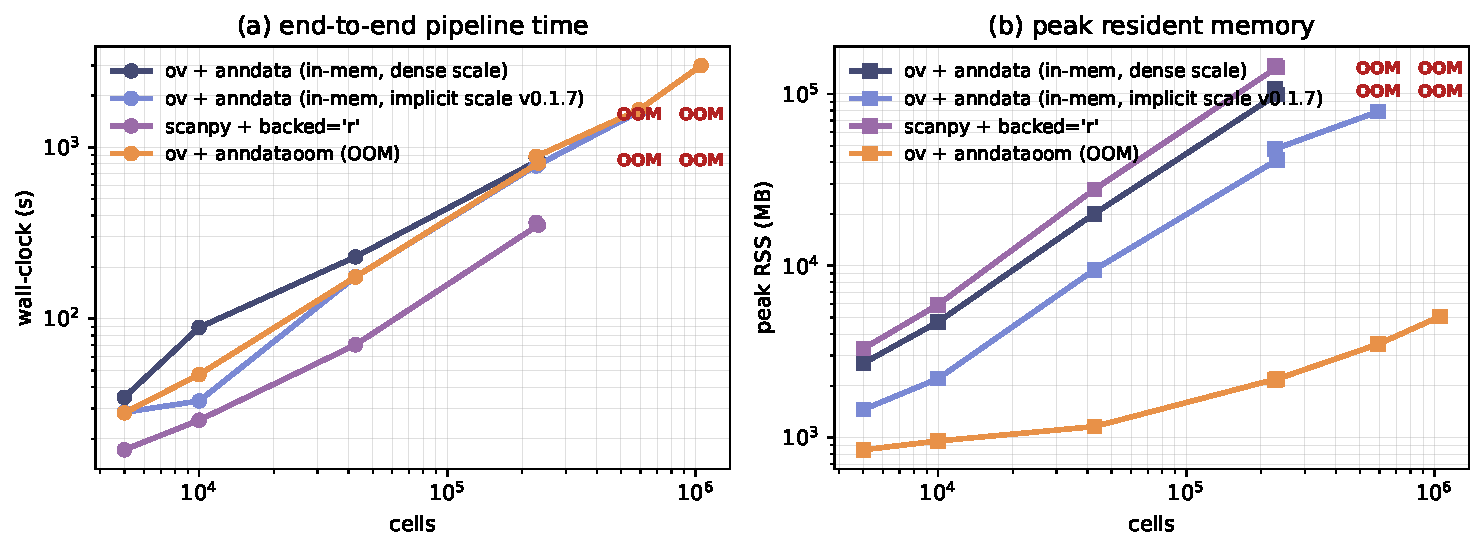
\includegraphics[width=\textwidth]{../figures/fig_totaltime.pdf}
  \caption{\textbf{Fig.~1 \textbar\ Memory and runtime scale differently
    across storage backends.} End-to-end pipeline wall-clock (left) and peak
    RSS (right) versus dataset size, log--log, for the four configurations.
    The out-of-memory backend's nearly flat RSS reflects chunk-bounded
    allocation; the in-memory backends grow linearly via the dense scaling
    step and are killed at the $\rssCapGB$~GB per-process cap for
    $\ge \firstOomSize$ cells (annotated ``OOM'').}
  \label{fig:totaltime}
\end{figure}

\begin{table}[t]
  \centering
  \caption{\textbf{Benchmark datasets.} Seven real Tabula Sapiens
    slices\cite{tabulasapiens2022} from cellxgene\cite{megill2021cellxgene}
    on the shared $60{,}606$-gene panel, with
    \texttt{layers["decontXcounts"]} (DecontX-decontaminated counts)
    promoted to \texttt{.X}.}
  \label{tab:datasets}
  \small
  \begin{tabular}{lrrrl}
\toprule
Dataset & Cells & Genes & On-disk (MB) & Source \\
\midrule
TS-5k & 5,000 & 60,606 & 130.1 & Tabula Sapiens vasculature (sub) \\
TS-10k & 10,000 & 60,606 & 222.5 & Tabula Sapiens vasculature (sub) \\
TS-Vasc & 42,650 & 60,606 & 2081.8 & Tabula Sapiens vasculature \\
TS-Stromal & 232,684 & 60,606 & 9594.1 & Tabula Sapiens stromal compartment \\
TS-Epi & 228,032 & 60,606 & 11066.5 & Tabula Sapiens epithelial compartment \\
TS-Immune & 592,317 & 60,606 & 18858.0 & Tabula Sapiens immune compartment \\
TS-1M & 1,053,033 & 60,606 & 15439.3 & Tabula Sapiens stromal+epi+immune (concat) \\
\bottomrule
\end{tabular}
\end{table}

\begin{table}[t]
  \centering
  \caption{\textbf{End-to-end wall-clock and peak RSS} for each
    (configuration, dataset) cell.
    ``\texttt{ov-anndata\textsuperscript{*}}'' denotes the implicit-centered
    scaling path. ``OOM'' marks runs killed by the $\rssCapGB$~GB
    per-process cap.}
  \label{tab:headline}
  \footnotesize
  \resizebox{\textwidth}{!}{\begin{tabular}{lrrrrrrrr}
\toprule
 & \multicolumn{2}{c}{\texttt{ov-anndata}} & \multicolumn{2}{c}{\texttt{ov-anndata\textsuperscript{*}}} & \multicolumn{2}{c}{\texttt{scanpy-backed}} & \multicolumn{2}{c}{\texttt{ov-oom}} \\
 & t (s) & RSS (MB) & t (s) & RSS (MB) & t (s) & RSS (MB) & t (s) & RSS (MB) \\
\midrule
TS-5k & 20.3 & 2711.5 & 19.6 & 1470.1 & 10.0 & 3300.6 & 36.9 & 866.7 \\
TS-10k & 32.2 & 4716.8 & 29.1 & 2213.7 & 14.9 & 5940.4 & 39.5 & 927.8 \\
TS-Vasc & 151.7 & 20095.3 & 151.2 & 9404.1 & 79.2 & 27821.5 & 151.9 & 1160.2 \\
TS-Stromal & 766.9 & 99371.0 & 745.9 & 41229.6 & 413.9 & 142962.9 & 668.5 & 2196.2 \\
TS-Epi & 880.1 & 106938.9 & 866.9 & 47831.9 & 375.8 & 146379.4 & 800.7 & 2017.6 \\
TS-Immune & OOM & -- & 1509.0 & 78949.4 & OOM & -- & 1476.6 & 3261.8 \\
TS-1M & OOM & -- & OOM & -- & OOM & -- & 2688.7 & 5168.7 \\
\bottomrule
\end{tabular}}
\end{table}

\subsection{Per-stage cost and numerical equivalence}

Decomposing by stage (Fig.~\ref{fig:stages}), the out-of-memory backend's
wall-clock is dominated by PCA, while the in-memory backends are dominated by
the dense scaling step and PCA. Normalisation and $\log(1{+}x)$ are
effectively free in the out-of-memory path because both are absorbed into the
lazy wrapper and execute only during the next consumer's chunked read. The
two backends produce identical principal components up to a per-component
sign flip inherent to the SVD: per-component cosine similarity
$\ge 0.9999$ on every dataset where both completed.

\begin{figure}[t]
  \centering
  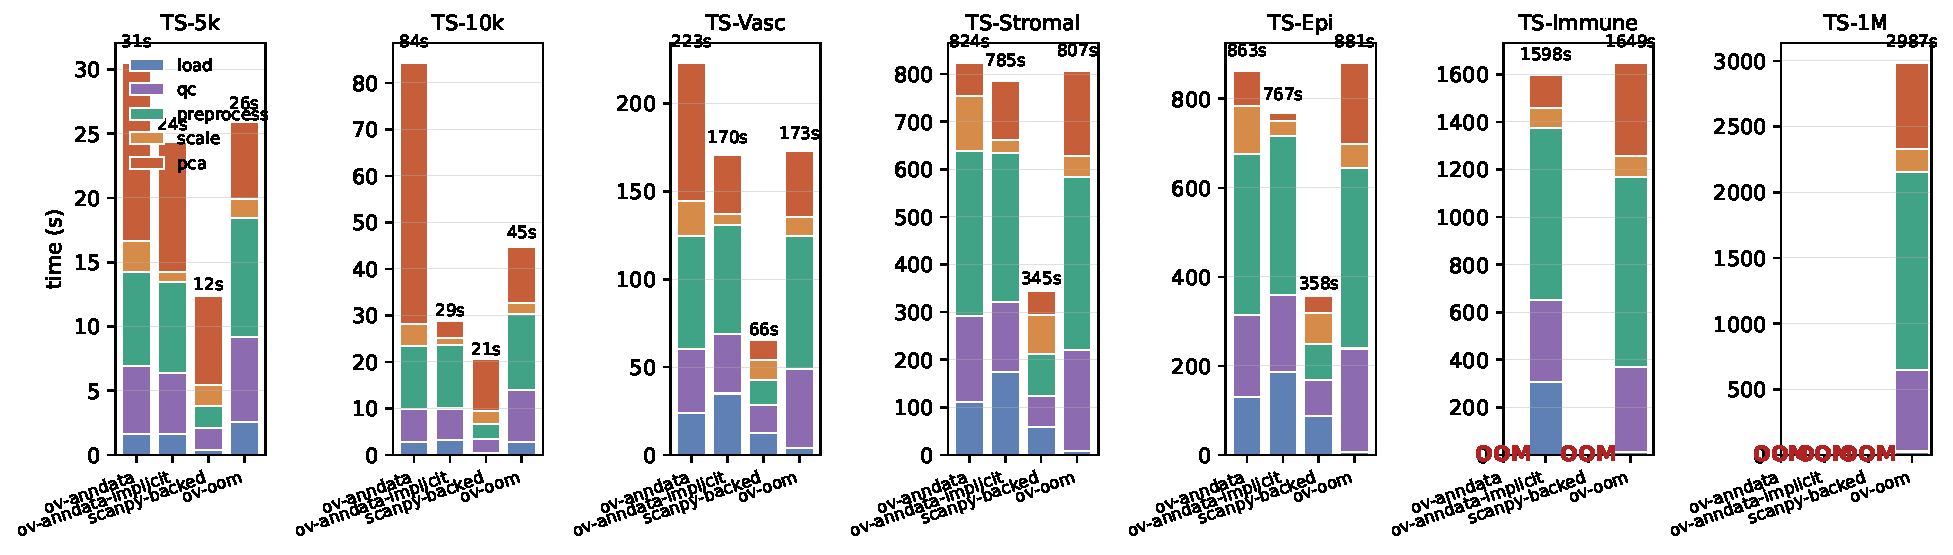
\includegraphics[width=0.95\textwidth]{../figures/fig_stages.pdf}
  \caption{\textbf{Fig.~2 \textbar\ Per-stage wall-clock breakdown} across
    all benchmark points. The out-of-memory \texttt{normalize} stage is
    effectively free; its cost is amortised into the next chunked read.}
  \label{fig:stages}
\end{figure}

\subsection{Composes with GPU-mixed execution at no penalty}

\texttt{omicverse} offers a \texttt{cpu-gpu-mixed} execution mode that
offloads PCA, neighbour-graph construction and embedding to a GPU through
PyTorch. Because \texttt{anndataoom} is a \emph{storage} backend and mixed
mode is a \emph{compute} mode, the two are orthogonal. Running the
out-of-memory pipeline under mixed mode on an NVIDIA H100, the
quality-control-to-PCA pipeline is \emph{mode-invariant}: at \mixedOomLabel\
($\mixedOomCells$ cells) wall-clock moves only $\mixedOomCpuSec\to\mixedOomMixSec$~s
and peak RSS is unchanged ($\mixedOomCpuRssGB$ vs $\mixedOomMixRssGB$~GB),
with \emph{no} GPU memory allocated during these stages
(Table~\ref{tab:mixed}). This follows structurally: the chunked operators are
CPU-resident, and the out-of-memory PCA dispatches to a chunked solver rather
than the GPU path, so the accelerator is never engaged for the
memory-bound work that the backend exists to make tractable --- and peak RSS
stays flat regardless of mode. GPU offload does engage for the downstream
graph and embedding steps, which operate on the compact
($n_\mathrm{obs}\times 50$) PCA embedding and never touch the matrix. On an
in-memory backend GPU offload of PCA gave no consistent speedup at these
scales, as the CPU covariance-eigendecomposition solver already completes the
$2{,}000$-HVG decomposition in well under ten seconds. The out-of-memory
backend therefore composes with mixed mode while preserving its flat-memory
guarantee.

\begin{table}[t]
  \centering\footnotesize
  \caption{\textbf{CPU vs CPU-GPU-mixed} on the out-of-memory and in-memory
    backends across scale. ``GPU (MB)'' is peak PyTorch device memory during
    the four-stage pipeline; it is $\approx 0$ for the out-of-memory backend
    because its PCA path is CPU-resident.}
  \label{tab:mixed}
  \resizebox{\textwidth}{!}{\begin{tabular}{llrrrrrr}
\toprule
Backend & Dataset & \multicolumn{2}{c}{cpu} & \multicolumn{3}{c}{cpu-gpu-mixed} & speedup \\
& & t (s) & RSS (MB) & t (s) & RSS (MB) & GPU (MB) & $t_{\mathrm{cpu}}/t_{\mathrm{mix}}$ \\
\midrule
OOM (anndataoom) & TS-5k & 28.3 & 847.0 & 26.1 & 922.1 & 0.0 & 1.08 \\
OOM (anndataoom) & TS-10k & 47.3 & 953.3 & 43.5 & 987.4 & 0.0 & 1.09 \\
OOM (anndataoom) & TS-Vasc & 175.3 & 1156.3 & 167.0 & 1140.0 & 0.0 & 1.05 \\
OOM (anndataoom) & TS-Stromal & 809.4 & 2196.4 & 859.7 & 2163.9 & 0.0 & 0.94 \\
OOM (anndataoom) & TS-Epi & 884.1 & 2166.5 & 935.2 & 2087.7 & 0.0 & 0.95 \\
OOM (anndataoom) & TS-Immune & 1653.5 & 3487.7 & 1637.3 & 3267.8 & 0.0 & 1.01 \\
OOM (anndataoom) & TS-1M & 2993.9 & 5061.1 & 3198.0 & 4941.7 & 0.0 & 0.94 \\
in-memory dense & TS-5k & 34.9 & 2701.2 & 21.5 & 3166.7 & 324.4 & 1.62 \\
in-memory dense & TS-10k & 89.0 & 4699.6 & 31.2 & 5123.9 & 400.7 & 2.85 \\
in-memory dense & TS-Vasc & 229.6 & 20077.7 & 165.9 & 20366.7 & 898.9 & 1.38 \\
in-memory dense & TS-Stromal & 837.9 & 99550.2 & 847.9 & 99161.5 & 3798.6 & 0.99 \\
in-memory dense & TS-Epi & 873.9 & 107061.8 & 943.4 & 106730.5 & 3728.1 & 0.93 \\
\bottomrule
\end{tabular}}
\end{table}

\subsection{Function coverage and cross-platform support}

Beyond the four pipeline stages, $\compatNOk$ of $\compatNFuncs$ probed
\texttt{omicverse.pp} functions run on the out-of-memory backend
(Table~\ref{tab:compat}), covering the full canonical workflow
(\texttt{qc}, \texttt{preprocess}, \texttt{normalize\_total},
\texttt{log1p}, \texttt{identify\_robust\_genes}, \texttt{scale},
\texttt{pca}) and the graph, clustering and embedding steps
(\texttt{neighbors}, \texttt{leiden}, \texttt{louvain}, \texttt{umap},
\texttt{tsne}, \texttt{mde}, \texttt{sude}). The remaining functions are not
yet wired through the backend-detection dispatch and raise a clear exception
at the call site rather than silently mis-computing. The Rust extension,
which links HDF5, builds and passes its test suite on Linux, macOS
(Apple-silicon and Intel) and Windows across Python 3.10 and 3.12 in
continuous integration.

\begin{table}[t]
  \centering\footnotesize
  \caption{\textbf{\texttt{omicverse.pp} compatibility} on the out-of-memory
    backend. \cmark\ = runs to completion; \xmark\ = raises (not yet
    backend-adapted); superscript \textsuperscript{G} marks a call that
    offloads to the GPU under \texttt{cpu-gpu-mixed}.}
  \label{tab:compat}
  \begin{tabular}{lcccr}
\toprule
\texttt{ov.pp} function & cpu & mixed & GPU-offload & note \\
\midrule
\texttt{qc} & \cmark & \cmark & -- &  \\
\texttt{preprocess} & \cmark & \cmark & -- &  \\
\texttt{scale} & \cmark & \cmark & -- &  \\
\texttt{pca} & \cmark & \cmark & -- &  \\
\texttt{neighbors} & \cmark & \cmark\,\textsuperscript{G} & yes &  \\
\texttt{leiden} & \cmark & \cmark & -- &  \\
\texttt{louvain} & \cmark & \cmark & -- &  \\
\texttt{umap} & \cmark & \cmark\,\textsuperscript{G} & yes &  \\
\texttt{tsne} & \cmark & \cmark & -- &  \\
\texttt{mde} & \cmark\,\textsuperscript{G} & \cmark\,\textsuperscript{G} & yes & torch (GPU-capable) \\
\texttt{sude} & \cmark & \xmark & -- & fails in mixed (NaN) \\
\texttt{normalize\_total} & \cmark & \cmark & -- &  \\
\texttt{log1p} & \cmark & \cmark & -- &  \\
\texttt{identify\_robust\_genes} & \cmark & \cmark & -- &  \\
\texttt{highly\_variable\_features} & \xmark & \xmark & -- & pegasus HVF densifies \\
\texttt{highly\_variable\_genes} & \xmark & \xmark & -- & standalone; use \texttt{preprocess} \\
\texttt{normalize\_pearson\_residuals} & \xmark & \xmark & -- & not OOM-adapted \\
\texttt{regress} & \xmark & \xmark & -- & scanpy regress\_out densifies \\
\texttt{scrublet} & \xmark & \xmark & -- & backed var lookup \\
\texttt{score\_genes\_cell\_cycle} & \xmark & \xmark & -- & backed var lookup \\
\texttt{filter\_cells} & \xmark & \xmark & -- & not OOM-adapted \\
\texttt{filter\_genes} & \xmark & \xmark & -- & not OOM-adapted \\
\texttt{anndata\_to\_GPU} & \xmark & \xmark & -- & needs rapids \\
\texttt{anndata\_to\_CPU} & \xmark & \xmark & -- & needs rapids \\
\bottomrule
\end{tabular}
\end{table}

\section{Discussion}

For real-data sizes from $5{,}000$ cells upward the out-of-memory backend
matches or beats the in-memory pipeline's wall-clock while using a small
fraction of the memory, because it avoids loading and densifying the full
gene panel; past the in-memory frontier it continues without intervention,
with peak RSS bounded by chunk size rather than by cell count. The cost is
that lazy, on-disk evaluation re-reads from disk at each stage, so for
workflows that fit comfortably in RAM and re-use a loaded \texttt{AnnData}
many times within a session, the amortised cost of the in-memory backend can
be lower. The backend is a storage-layer change only --- it does not alter
the analysis or its numerics --- so it composes with GPU-accelerated compute
and with the broader \texttt{omicverse} ecosystem. The natural extensions are
broader backend-adapted coverage of auxiliary functions, and multi-omic
layers (ATAC peaks, protein counts) following the same lazy-wrap pattern.

\section{Methods}

\paragraph{Storage and transform layer.} The h5ad reader is the
\texttt{anndata-rs} Rust library, exposed to Python as a \texttt{BackedArray}
proxy. Per-cell normalisation is implemented as left multiplication by a
sparse diagonal of inverse size factors; $\log(1{+}x)$ is applied to the
sparse values only. Per-gene mean and variance for scaling are computed in a
single chunked pass using a hybrid estimator: per-chunk statistics use the
sparse-native $E[X^2]-E[X]^2$ identity, and cross-chunk accumulation uses
Welford's method\cite{welford1962numerically} on the per-chunk mean and
sum-of-squared-deviations, keeping the numerical error at the
\texttt{float32}$\to$\texttt{float64} accumulation floor
($\sim$$7\times10^{-8}$ relative).

\paragraph{Chunked PCA.} Dimensionality reduction uses a randomised
SVD\cite{halko2011randomsvd} over the lazy scaled matrix. When the post-HVG
matrix fits a configurable memory budget it is built once into RAM and
factorised in a single pass; otherwise an implicit-centered formulation
rewrites the matrix--vector products through the identity
$(N-\mu)/\sigma\cdot W = N\cdot\mathrm{diag}(1/\sigma)\cdot W -
(\mu/\sigma)\cdot W$, where $N$ is the sparse normalise+$\log(1{+}x)$ view,
so no dense per-chunk block is allocated. When the matrix is materialised,
HVG columns are sliced from the sparse parent \emph{before} densifying ---
since normalisation is per-row and $\log(1{+}x)$ is element-wise, the column
slice commutes through both --- so only a $(\mathrm{chunk}\times n_\mathrm{HVG})$
block is ever dense; this is numerically identical to densifying the full
panel (maximum absolute difference $\sim$$10^{-7}$).

\paragraph{Benchmark configurations.} \texttt{ov-anndata}: input loaded with
\texttt{anndata.read\_h5ad}; \texttt{ov.pp.scale} densifies the full panel.
\texttt{ov-anndata-implicit}: as above but \texttt{ov.pp.scale} stores the
scaled matrix as a sparse-backed implicit-centered wrapper.
\texttt{scanpy-backed}: input opened \texttt{backed='r'}, then the standard
scanpy pipeline; because the first quality-control operation has no handler
for the backed dataset type, the workflow materialises to memory before QC,
so the backed advantage exists only at load. \texttt{ov-oom}: input opened
with \texttt{anndataoom.read}; operations dispatch to the chunked path via
\texttt{is\_oom}.

\paragraph{Datasets.} Seven Tabula Sapiens slices\cite{tabulasapiens2022}
from cellxgene\cite{megill2021cellxgene} on the shared $60{,}606$-gene panel:
TS-Vasculature ($42{,}650$ cells) and two random subsamples ($5{,}000$ /
$10{,}000$, seed 0); the stromal ($232{,}684$), epithelial ($228{,}032$) and
immune ($592{,}317$) compartments; and a one-million-cell concatenation
($\oneMCells$ cells). Each input uses \texttt{layers["decontXcounts"]} as
\texttt{.X}; the harness promotes the raw-counts layer when \texttt{.X}
appears log-normalised, to avoid double-normalisation.

\paragraph{Measurement.} Per-stage wall-clock and RSS are captured around
each pipeline stage (peak RSS reported as the maximum post-stage RSS).
The main sweep runs on a single CPU node under a $\rssCapGB$~GB per-process
cap; the GPU-mixed comparison runs on an NVIDIA H100 node, recording per-stage
peak PyTorch device memory in addition to RSS. Numerical equivalence is
quantified by per-component absolute cosine similarity between backends.

\paragraph{Code and data availability.} The benchmark harness, figure/table
generators and dataset cards are at the project
repository\cite{anndataoom}. Subsamples use a fixed seed; the
million-cell input is the row-concatenation of the three compartment slices.

\bibliographystyle{unsrtnat}
\bibliography{references}

\end{document}
